%!TEX root = ../../main.tex
\chapter{Theoretische Grundlagen}
\section{Künstliche Intelligenz}
\ac{KI} wird zunehmend in verschiedenen Bereichen eingesetzt und erleichtert die Arbeit der Menschen enorm. Viele Arbeiten können mit Hilfe von \ac{KI} schneller und besser erledigt werden. Im folgenden Abschnitt werden die Begriffe 'Intelligenz' und 'Künstliche Intelligenz' erläutert, um ein einfaches Verständnis zu schaffen. Außerdem werden die verwandten Begriffe Machine Learning und Deep Learning in den Kontext eingeordnet.

In der Psychologie bezieht sich Intelligenz auf die Fähigkeit, logische, sprachliche, mathematische oder sensorische Probleme zu lösen, aber es gibt keine allgemeingültige Definition von Intelligenz. Die kognitiven Fähigkeiten des Menschen ermöglichen es ihm, sich an Beschreibungen oder Erklärungen von Dingen zu erinnern, die er zu einem späteren Zeitpunkt wieder abrufen und verwenden kann. Das menschliche Gehirn, das aus Milliarden von Neuronen besteht, lernt und speichert bestimmte Strukturen, Konzepte und Fähigkeiten. Beim Lernen werden die Verbindungen zwischen den Neuronen im Gehirn verstärkt. Je öfter etwas gelernt wird, desto stärker werden bestimmte Verbindungen zwischen den Neuronen im Gehirn. \cite[vgl.][]{Ertel2021,Posthoff2022}

Künstliche Intelligenz hingegen ist ein Wissenschaftsgebiet, das sich damit beschäftigt, Computern menschliches Verhalten beizubringen. Damit ist gemeint, dass ein Computer darauf trainiert wird, ähnlich wie ein Mensch zu denken und entsprechend zu handeln. \cite[vgl.][]{Lang2023} Im Gegensatz zu biologischen Neuronen lösen Computer Probleme wie die Klassifizierung eines Bildes durch die Anwendung mathematischer Funktionen und Algorithmen. Es wird versucht, die Denkfähigkeit des Menschen nachzuahmen, um einen Mehrwert bei der Problemlösung durch Computer zu erzielen. Mit Hilfe der künstlichen Intelligenz sind Computer heute in der Lage, Probleme zu lösen, die früher ein höheres intellektuelles Verständnis erforderten. Computer können beispielsweise Bilder klassifizieren oder Vorhersagen treffen. Ähnlich wie der Mensch lernt auch der Computer aus den vorhandenen Daten und verstärkt dabei bestimmte mathematische Zusammenhänge. \cite[vgl.][]{WasIstKi}

\begin{figure}[h]
	\centering
	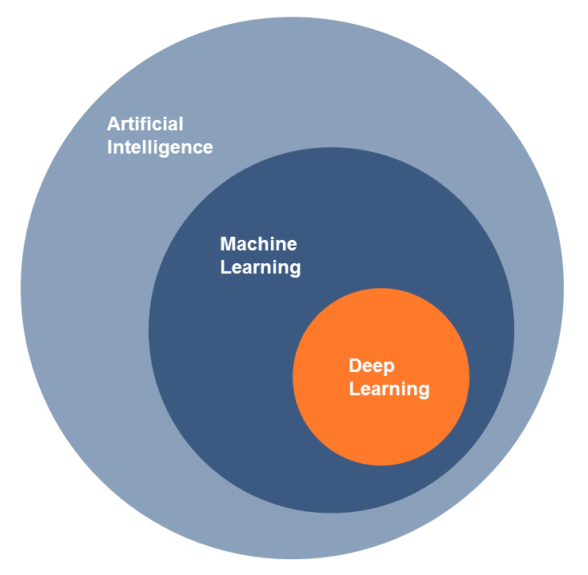
\includegraphics[height=.7\textwidth]{ai_overview.png}
	\caption{Übersicht der Bereiche von künstlicher Intelligenz (Quelle: \url{https://www.alexanderthamm.com/de/blog/ki_artificial-intelligence-ai-kuenstliche-neuronale-netze-machine-learning-deep-learning/})}
\end{figure}

Im Zusammenhang mit \ac{KI} wird häufig auch von Machine Learning, Deep Learning und Neuronalen Netzen gesprochen. \ac{KI} ist der Oberbegriff, der sowohl Machine Learning als auch Deep Learning umfasst. Deep Learning ist ein Teilbereich des Machine Learning, bei dem künstliche neuronale Netze zum Einsatz kommen, die es Computern ermöglichen, Dinge zu lernen und Probleme zu lösen. Im Folgenden wird der Schwerpunkt auf den Bereich Deep Learning gelegt.